%
% $Id: singlesection.tex,v 1.1 2010/09/18 02:48:07 livesey Exp $    
%
% This is the master file for the EOS MLS Level 2 v1.5 report.
%
\documentclass[portrait,twoside,11pt]{report}
\usepackage{newlargemls}
\usepackage[mtbold,mtplusscr,mtpluscal]{mathtime}
\usepackage{times}
\usepackage{pstcol,pst-node,pst-text}
\usepackage{graphicx}
\usepackage{verbatim,array}
\usepackage[square]{natbib}
\usepackage{pifont}
\usepackage{rotating}
\usepackage{amsmath}
\usepackage{multicol}
\usepackage{booktabs}
\usepackage{colortbl}
\usepackage{xr}
\usepackage[letterpaper,breaklinks,bookmarksopen=true,linktocpage=true]{hyperref}
% \newcommand{\UnderscoreCommands}{\do\dontincludegraphics}
% \usepackage[strings]{underscore}
% Use underscore in text mode
%
%
% Skip the include graphics possibly
% \renewcommand{\dontincludegraphics}[2][1]{}
%
%-------------------------------------------------------------------------------
%
% Now begin the document and set a few various counters and values etc.
%
\begin{document}
\rcsParseName $Name:  $
\rcsInfo $Id: singlesection.tex,v 1.1 2010/09/18 02:48:07 livesey Exp $
%
\setcounter{tocdepth}{2}
\setlength{\itemsep}{0pt}
\setlength{\parsep}{0pt}
\bibliographystyle{plainnat}
%
% Define various macros
%
\renewcommand{\b}{\mathbf}
\newcommand{\T}{^{\text{T}}}
\newcommand{\cs}[1]{\ensuremath{_{\text{#1}}}}
\newcommand{\inv}{^{\mathrm -1}}
\newcommand{\cp}[1]{\ensuremath{^{\text{#1}}}}
\newcommand{\degsym}{\ensuremath{^\circ}}
%
%
\newcommand{\mycomment}[1]{{\small\sffamily\color{red}\slshape[#1]}}
%
% These rather complex beasties are the various macros used to make up
% The information on a product.

% ---------------------------------------- Defining a product
% This command sets up a section for a species.
%
\newcommand{\thumbmark}{}
\newcommand{\thumbbackground}{black}
%
\newcommand{\speciestitle}[5][]{%
\cleardoublepage\suppressfloats[t]
\renewcommand{\thumbmark}{#3}%
\addtolength{\thumbpos}{-0.45in}%
\section{#2}
\begin{description}
\item[Swath name:] \texttt{#4} #1
#5
\end{description}}
%
\newlength{\thumbpos}
\newcommand{\makethumbmark}[2]{%
  \begin{tikzpicture}[overlay]
    \node at (#1,\thumbpos) [rotate=#2,anchor=south]
    {\colorbox{black}{\parbox{1.5cm}{\centering%
        \color{white}\sffamily\bfseries\large\selectfont\rule[-0.5ex]{0pt}{2ex}\thumbmark}}};%
  \end{tikzpicture}}
%
\newcommand{\startthumbmarks}{%
  \setlength{\thumbpos}{9.2in}%
  \lfoot[\makethumbmark{-1cm}{90}\thepage]{\myshorttitle}%
  \rfoot[Aura Microwave Limb Sounder]{\thepage\makethumbmark{1cm}{-90}}%
} \newcommand{\killthumbmarks}{%

  \lfoot[\thepage\hspace{1cm}\tinyrcs]{\myshorttitle} % should be \@shortitle
  \rfoot[EOS Microwave Limb Sounder]{\tinyrcs\hspace{1cm}\thepage}}
\newcommand{\email}[1]{\textbf{Email:} $<$\texttt{#1}$>$}
%
% Change the figures/table counters
\makeatletter
\def\renewcounter#1{%
    \@ifundefined{c@#1}
    {\@latex@error{counter #1 undefined}\@ehc}%
    \relax
    \let\@ifdefinable\@rc@ifdefinable
    \@ifnextchar[{\@newctr{#1}}{}}
\makeatother
\renewcounter{figure}[section]
\renewcounter{table}[section]
\renewcommand{\thefigure}{\thesection.\arabic{figure}}
\renewcommand{\thetable}{\thesection.\arabic{table}}
%
\newcommand{\screeningrule}[1]{\textbf{#1}\par}

% -------------------------- Averaging kernels
\newcommand{\extracaption}{}

\newcommand{\avkcaption}[2]{%
  Typical two-dimensional (vertical and horizontal along-track)
  averaging kernels for the MLS \thisv #2#1 data at 70\degsym N (upper)
  and the equator (lower); variation in the averaging kernels is
  sufficiently small that these are representative of typical profiles.
  Colored lines show the averaging kernels as a function of MLS
  retrieval level, indicating the region of the atmosphere from which
  information is contributing to the measurements on the individual
  retrieval surfaces, which are denoted by plus signs in corresponding
  colors.  The dashed black line indicates the resolution, determined
  from the full width at half maximum (FWHM) of the averaging kernels,
  approximately scaled into kilometers (top axes).  (Left) Vertical
  averaging kernels (integrated in the horizontal dimension for five
  along-track profiles) and resolution.  The solid black line shows the
  integrated area under each kernel (horizontally and vertically);
  values near unity imply that the majority of information for that MLS
  data point has come from the measurements, whereas lower values imply
  substantial contributions from a priori information.  (Right)
  Horizontal averaging kernels (integrated in the vertical dimension)
  and resolution.  The horizontal averaging kernels are shown scaled
  such that a unit averaging kernel amplitude is equivalent to a factor
  of 10 change in pressure.}

\newcommand{\vertavkcaption}[2]{%
  Typical vertical averaging kernels for the MLS \thisv #2#1 data at
  70\degsym N (left) and the equator (right); variation in the averaging
  kernels is sufficiently small that these are representative of typical
  profiles.  Colored lines show the averaging kernels as a function of
  MLS retrieval level, indicating the region of the atmosphere from
  which information is contributing to the measurements on the
  individual retrieval surfaces, which are denoted by plus signs in
  corresponding colors.  The dashed black line indicates the vertical
  resolution, determined from the full width at half maximum (FWHM) of
  the averaging kernels, approximately scaled into kilometers (top
  axes).  The solid black line shows the integrated area under each
  kernel; values near unity imply that the majority of information for
  that MLS data point has come from the measurements, whereas lower
  values imply substantial contributions from a priori information.  The
  low signal to noise for this product necessitates the use of
  significant averaging (e.g., monthly zonal mean), making horizontal
  averaging kernels largely irrelevant.}

\newcommand{\onestandardavk}[2]{%
\begin{figure}%
\begin{center}%
\includegraphics[width=0.8\linewidth]{figures/avk-#1}%
\end{center}
\caption{\avkcaption{#2}{}\extracaption}
\label{fig:Avk#1}%
\end{figure}}

\newcommand{\oneverticalavk}[2]{%
\begin{figure}%
\begin{center}%
\includegraphics[width=0.8\linewidth]{figures/avk-#1}%
\end{center}
\caption{\vertavkcaption{#2}{}\extracaption}
\label{fig:Avk#1}%
\end{figure}}

% ------------------------------------ Other boilerplate
\newcommand{\standardrangestatement}{Values outside this range are not
  recommended for scientific use.}
\newcommand{\standardprecisionrule}{%
\item[Estimated precision:] \screeningrule{Only use values for which the
    estimated precision is a positive number.} Values where the \emph{a
    priori} information has a strong influence are flagged with negative
  precision, and should not be used in scientific analyses (see
  Section~\ref{sec:NegativePrecision}).}
\newcommand{\evenstatusrule}{%
\item[Status flag:] \screeningrule{Only use profiles for which the
    `Status' field is an even number.}  Odd values of \texttt{Status}
  indicate that the profile should not be used in scientific studies.
  See Section~\ref{sec:StatusQuality} for more information on the
  interpretation of the \texttt{Status} field.}
\newcommand{\cloudsokrule}{\screeningrule{%
    Profiles identified as being affected by clouds can be used with no
    restriction.}}
\newcommand{\qualityrule}[1]{\screeningrule{Only
    profiles whose `Quality' field is greater than #1 should be used.}}
\newcommand{\convergencerule}[1]{\screeningrule{Only profiles whose
    `Convergence' field is less than #1 should be used.}}

% ----------------------------------- Table flipflopping
\colorlet{tableoddbackground}{black!10}
\colorlet{tableevenbackground}{white}
\newif\ifoddrow\oddrowtrue
\newcommand{\flipfloprow}{%
  \ifoddrow
  \rowcolor{tableoddbackground}
  \global\oddrowfalse
  \else
  \rowcolor{tableevenbackground}
  \global\oddrowtrue
  \fi}
\newcommand{\samecolorrow}{%
  \ifoddrow
  \rowcolor{tableevenbackground}
  \else
  \rowcolor{tableoddbackground}
  \fi}  

%%% Local Variables: 
%%% mode: latex
%%% TeX-master: "v4-x-report"
%%% End: 

%
\newlength{\tablecaptionsep}
\setlength{\tablecaptionsep}{0.5ex}
%
\newcommand{\citenumfont}{\itshape}
%
\setcounter{chapter}{3}
\pagestyle{fancy}
\chapter{Results for `standard' MLS data products}
%
\speciestitle{Carbon monoxide}{CO}{CO}{
  \item[Useful range:] 215--0.001\,hPa
  \item[Contact:] Hugh C. Pumphrey (stratosphere/mesosphere), \email{H.C.Pumphrey@ed.ac.uk} \\ Michael Schwartz (troposphere), \email{Michael.J.Schwartz@jpl.nasa.gov}}

\subsection{Introduction}

Carbon monoxide is retrieved from radiance measurements of two bands in the MLS 240\,GHz radiometer. Full details are given in \citet{PumphreyEtal:2007} and \citet{LiveseyEtal:2008}.

\subsection{Differences between \thisv and \prevv}
The \thisv carbon monoxide (CO) product is extremely similar to the \prevv product, and both are very similar to v04.2x in the upper troposphere and stratosphere, with improvement in some cases relative to v4.2x in the mesosphere and mesopause region, which results from the use of a more computationally expensive, nonlinear forward model for radiances near the 230-GHz line center. Small differences between \thisv and \prevv CO in the upper stratosphere result from changes in the temperature and pointing retrieval, discussed in Section~\ref{sec:StandardTemperature}. 

In the upper mesosphere, \thisv and \prevv CO are less tightly constrained to the \emph{a priori} than is v04.2x CO (\emph{a priori} precision is 1.5$\times$ larger at 0.046\,hPa and 2$\times$ larger at and above 0.01\,hPa). Horizontal smoothing of \thisv has been tightened at and above 0.01\,hPa to maintain retrieval stability, but this change has no appreciable impact on the sharpness of horizontal features seen in preliminary validation. The top of the vertical range of the retrieval remains 0.00046\,hPa and profiles are recommended for scientific use up to 0.001\,hPa.

Figure~\ref{fig:CO_scatv6v5} shows scatter plots of screened \prevv vs.\ \thisv CO from 215\,hPa to 0.01\,hPa during 2009, showing that the two versions are almost identical. 
High outlier values of CO along the 1:1 lines of panels for 216--46.4\,hPa in Figure~\ref{fig:CO_scatv6v5} are measurements within the plume from the ``Black Saturday'' Australian wildfires and confirm the consistency of the \thisv and \prevv retrievals in the upper troposphere and lower stratosphere, even when unusally high values are retrieved .

The calculation of cloud flags bits in the product status has changed significantly in \thisv, as is discussed in Section~\mycomment{Point to appropriate section}.  \Thisv CO has approximately twice as many profiles marked as possibly influenced by low cloud than \prevv, and no profiles flagged as influenced by only high clouds.  Neither of these flags is used in the recommended screening.
\subsection{Resolution}
\onestandardavk{CO}{CO}%

Figure~\ref{fig:AvkCO} shows the horizontal and vertical averaging kernels for \thisv MLS CO\@. Estimated vertical and horizontal resolutions are essentially identical to those of \prevv and v04.2x. The vertical resolution is in the range 3.5--5\,km from the upper troposphere to the lower mesosphere, degrading to 6--7\,km in the upper mesosphere. Down to the 215\,hPa level, the vertical averaging kernels are sharply peaked at the level being retrieved, but while the \mbox{316-hPa} measurement contains contribution from 316\,hPa, it has a larger contribution from 215\,hPa and a negative contribution around 100\,hPa of similar magnitude to that at 316\,hPa. The retrieved value at 316\,hPa is thus more an extrapolation of the profile higher in the UTLS than it is an independent measurement at 316\,hPa, and it is not recommended for scientific use. The horizontal resolution is about 200\,km in the mesosphere, degrading slowly to 300\,km with decreasing height in the stratosphere and more rapidly to about 460\,km at 100\,hPa and 690\,km at 215\,hPa.

\begin{figure}
  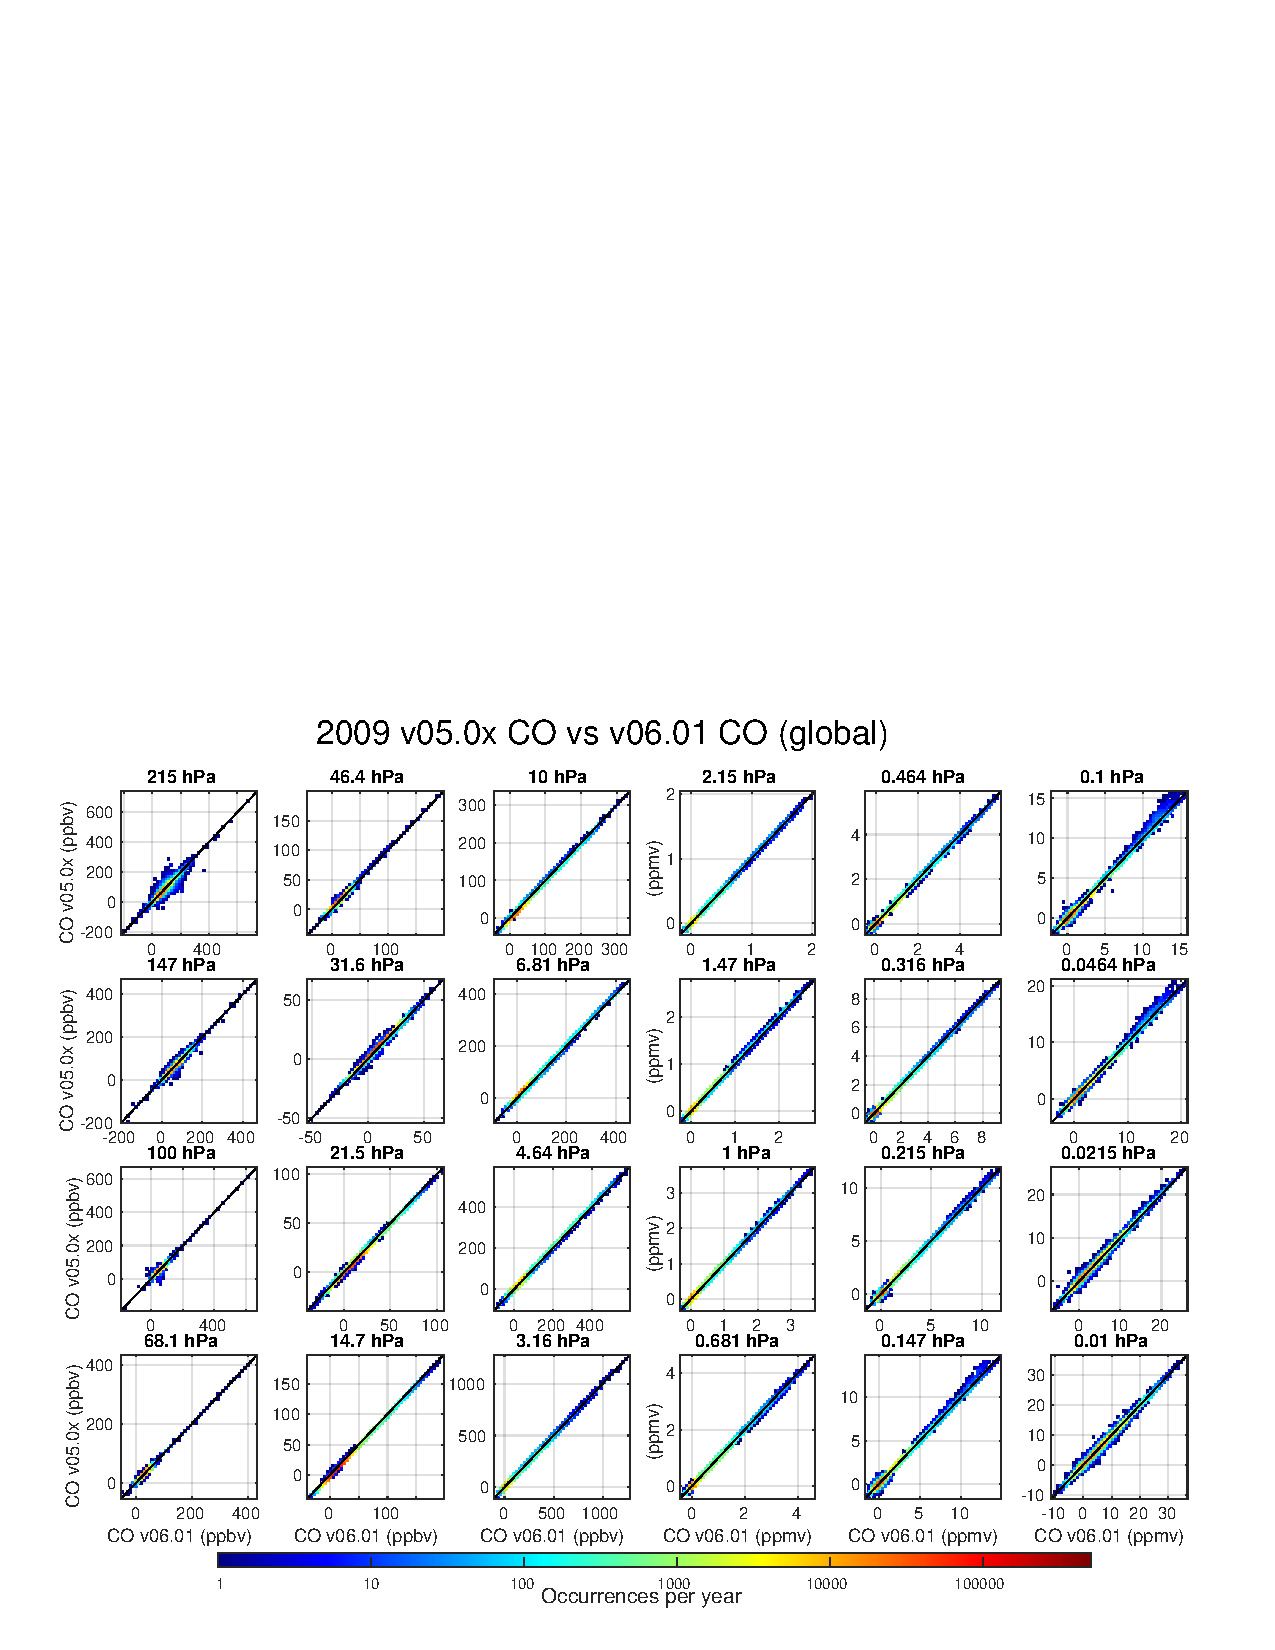
\includegraphics[width=\textwidth, trim=1.4cm 1cm 1.8cm 12.5cm]{figures/CO_scatv6v5}
  \caption{Joint histograms of \prevv CO and \thisv CO for 2009 data show the general consistency of the two versions.  The color scale is logarithmic, with red points along the 1:1 line corresponding to pairs of values that are identical in the two versions. }
  \label{fig:CO_scatv6v5}
\end{figure}

\subsection{Precision}

The MLS data are supplied with an estimated precision (the field \texttt{L2gpPrecision}) which is the \emph{a posteriori} precision as returned by the optimal estimation. The precision of the \thisv CO is nearly identical to that of \prevv, and very similar to that of v04.2x. Reported precision is greater than the scatter observed in the data in regions of low natural variability. This can be seen in the middle (low-latitude) panels of the second row of Figure~\ref{fig:COplot1bylat_log}, where the purple and yellow solid lines (scatter about the zonal means) have smaller values than the purple and yellow dashed lines (precisions). Where the estimated precision is greater than 50\% of the \emph{a priori} precision the data will be influenced by the \emph{a priori} to an undesirably large extent. In such cases, \texttt{L2gpPrecision} is set to be negative (or zero in some cases) to indicate that the data should not be used. The \thisv\mycomment{Verify this?} \emph{a priori} precision has been relaxed above 0.1\,hPa (blue dashed line departing from red dashed line in center panels of Figure~\ref{fig:COplot1bylat_log}), and the level at which the retrieved precision is more than half of this \emph{a priori} precision typically moves up from 0.0046\,hPa to 0.00046\,hPa.

\begin{figure}
  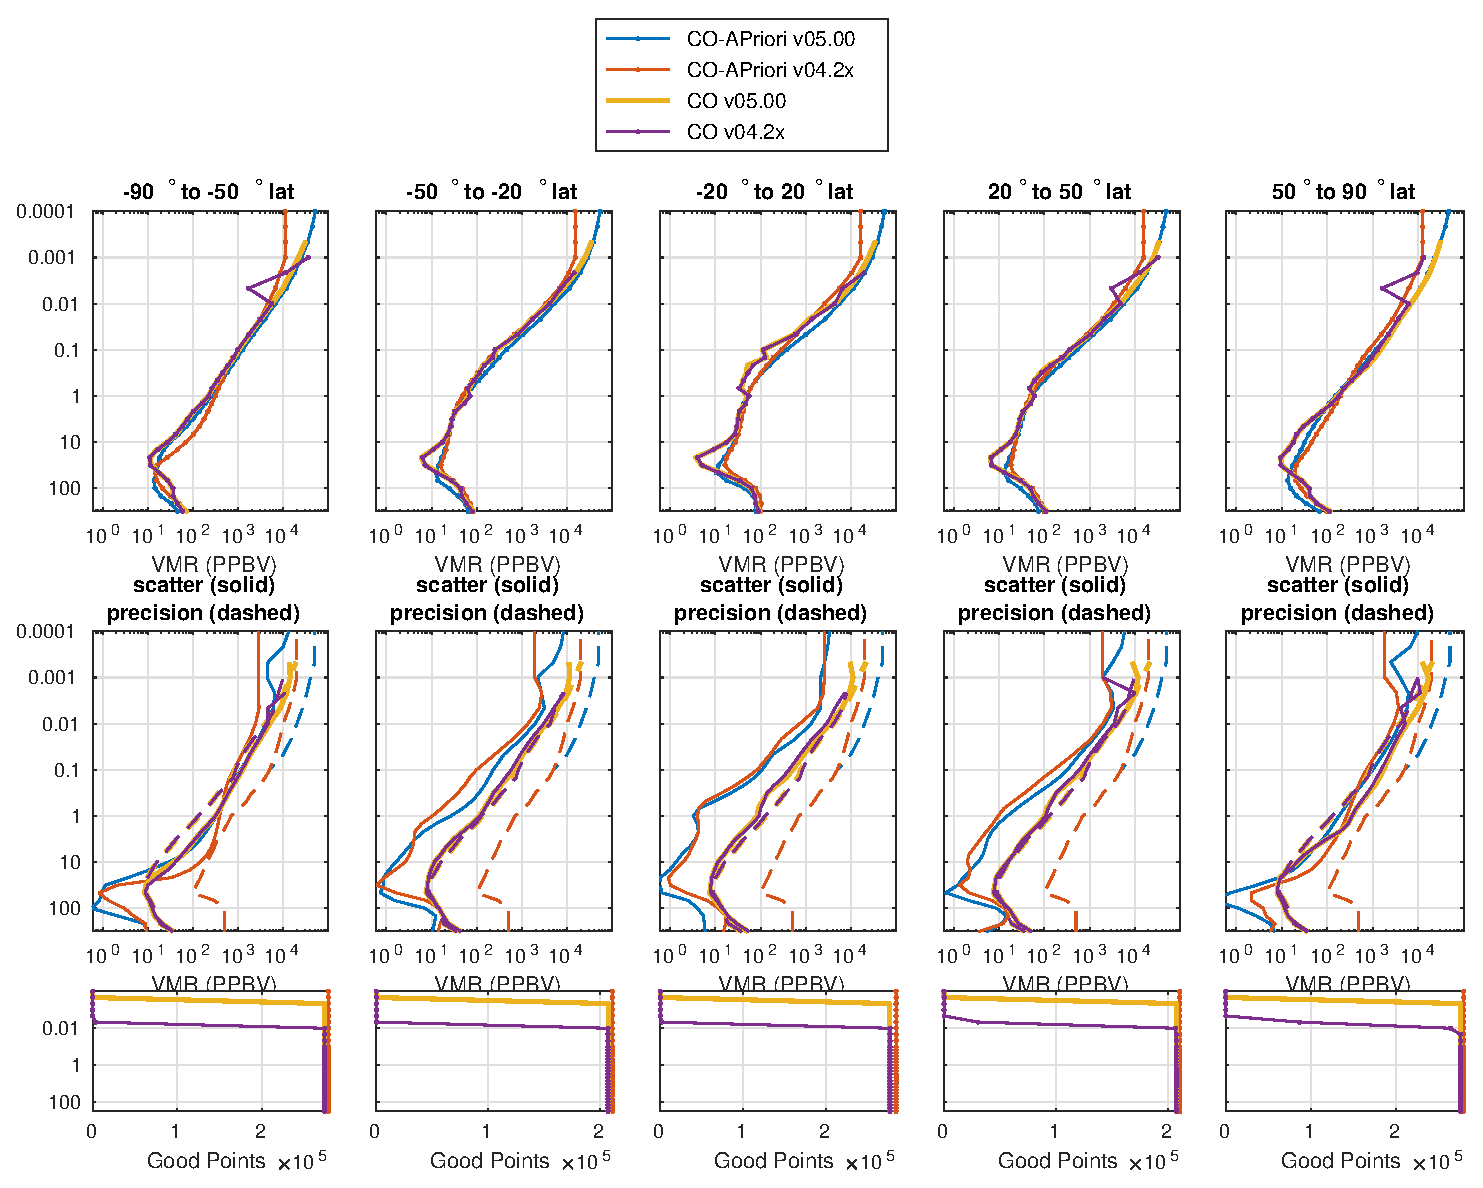
\includegraphics[width=\textwidth]{figures/COplot1bylat_log}
  \caption{\mycomment{This figure is still old, right?} The top row shows 2009 zonal means of \thisv\CheckThis and \prevv\CheckThis mixing ratios and their \emph{a priori} values.  The \prevv\CheckThis retrieved mixing ratio line (purple) lies on top of the \thisv\CheckThis mixing ratio line (yellow) for all but the highest altitude pressure surfaces, despite significant differences in their \emph{a priori} profiles. The middle row shows the zonal scatter about these zonal means (solid lines) and corresponding estimated precisions (dashed lines).  The bottom row shows the number of good profiles, limited at the highest retrieval levels where retrieved precision exceeds half of the \emph{a priori} precision.}
  \label{fig:COplot1bylat_log}
\end{figure}

Note that the random errors (precisions) are larger than 100\% of the mixing ratio for much of the vertical range, meaning that significant averaging (e.g., daily zonal mean or weekly map) is typially needed to make use of the data.

\subsection{Accuracy}
The estimated accuracy is summarized in Table~\ref{tab:COSummary}. In the middle atmosphere the accuracies are estimated by comparisons with the ACE-FTS instrument; see \citet{PumphreyEtal:2007} for further details. The MLS v2.2 CO data at 215\,hPa showed high (factor of \mytexttilde2) biases compared to other observations. The morphology, however, was generally realistic \citep{LiveseyEtal:2008}. In \thisv (as in \prevv) this bias has been essentially eliminated through a change in the approach to modeling the background radiance upon which the CO spectral line sits, and a small reduction in the number of MLS spectral channels considered in the retrieval. Tropospheric (215--100\,hPa) accuracies in Table~\ref{tab:COSummary} are 2-$\sigma$ estimates obtained by propagating parameter uncertainties through a model of the measurement system, and are unchanged from those calculated for \prevv.

\subsection{Data screening}
\label{sec:COScreening}
\begin{description}
  \item[Pressure range:] \screeningrule{215--0.001\,hPa.} \standardrangestatement\ Data at 0.00046\,hPa represents a total column at and above that pressure level. Scientific use of these 0.00046\,hPa data may be possible, but consultation with the MLS team is advised. \standardprecisionrule \evenstatusrule

  \item[Clouds:] Clouds have no impact for pressures of 31\,hPa or less. \thisv, \prevv and v04.2x CO are much less susceptible to cloud-induced artifacts than was v03.x, so screening of the CO product is considerably simplified compared to that recommended for v03.x, needing only application of the standard \texttt{Quality} and \texttt{Convergence} rules as described below. The low-cloud status bit, which was set for 0.2\% of profiles in \prevv, is set for 0.6\% of profiles in \thisv, but preliminary validation does not find this flag to be useful for data screening.

  \item[Quality:] \screeningrule{Only use profiles with \texttt{Quality} greater than 1.5.} Profiles with \texttt{Quality} less than or equal to 1.5 comprise 0.7\% of all data, and \mytexttilde2\% of profiles in the tropics. At 215 hPa in the tropics, the rejected profiles have mixing ratios that are, on average, 7\% higher than other tropical values and the occurrence rates of high outliers with mixing ratios greater than 150\,ppbv is about twice that of the rest of the tropical ensemble. At 100\,hPa there is no significant difference in the means of tropical profiles with Quality less than or greater than 1.5.

  \item[Convergence:] \convergencerule{1.03} This \texttt{Convergence} criterion rejects fewer than 0.1\% of profiles. Almost all of the retrievals in the phase that produces \thisv CO converge to their target, so \texttt{Convergence} is of limited use in screening.
\end{description}

\subsection{Artifacts}
\begin{itemize}
  \item Positive systematic error of 20--50\% throughout the mesosphere, as was the case for \prevv.
  \item Negative systematic error of 50--70\% near 30\,hPa, as was the case for \prevv.
  \item Retrieved profiles are rather jagged, especially between 1\,hPa (48\,km) and 0.1\,hPa (64\,km). The greater smoothing applied in \thisv, \prevv, v04.2x and v03.3 compared to v2.2 reduced this problem considerably but has not eliminated it entirely.
  \item The tendency for negative values to occur at the level below a large positive value that was present in v04.2x is somewhat reduced in \thisv and \prevv.
  \item Upper-tropospheric \thisv CO retrieved values still show some anomalous sensitivity to thick clouds associated with deep convection. The screening procedure based upon \texttt{Quality} and \texttt{Convergence} that is described above is generally effective in removing these artifacts.
  \item Negative outliers in UT CO have been observed in volcanic plumes, such as that from the eruption of Sarychev in June of 2009. These are likely the result of interference from spectral lines of a gas-phase plume component, and are a subject for further analysis and validation.
\end{itemize}

\subsection{Review of comparisons with other datasets}

In the upper troposphere, comparisons with various in situ CO observations (NASA DC-8, WB-57 and the MOZAIC dataset) indicate that the \emph{earlier} MLS v2.2 215\,hPa CO product was biased high by a factor of \mytexttilde2. As in v04.2x and \prevv, this bias is largely eliminated in \thisv.

In the mesosphere, comparisons of the earlier v2.2 MLS CO with ODIN-SMR and ACE-FTS suggest a positive bias: 30\%--50\% against ACE-FTS, 50\%--100\% against SMR. Near 31\,hPa, the MLS values are lower than SMR and ACE-FTS by at least 70\%. The MLS values have not changed much between v2.2 and \thisv in the middle atmosphere, so these comparisons may mostly be considered valid for \thisv. What change there was between v2.2 and later versions consists of a slight lowering of the MLS values, bringing them slightly towards the ACE-FTS data; 20\% is now a better estimate of the MLS-ACE bias in much of the middle atmosphere (compared to 30\% with v2.2).
% Mean difference between \prevv\CheckThis and \thisv\CheckThis in the lower mesosphere
% are still generally small.
Further validation of the \thisv retrieval above 0.01\,hPa is needed.

\begin{table}
  \caption{Data quality summary for MLS \thisv CO.}
  \vspace{\tablecaptionsep}
  \label{tab:COSummary}
  \begin{minipage}{\linewidth}
    \centering\begin{tabular}{ccccl}
\toprule
\textbf{Pressure} &
\textbf{Resolution / km} & 
\textbf{Precision} / &
\textbf{Accuracy} &  
\textbf{Comment} \\
\textbf{/ hPa} &
\textbf{Vert $\times$ Horiz.} &
\textbf{ppbv} \\
\midrule
$<0.001$  &    ---        &   ---   &    ---      & Not retrieved\\
0.00046  & ---       &   ---   &    ---    & Unsuitable
for scientific use \\
0.001  &   7.2   $\times$ 200 &  12000  & validation needed & possibly use, with caution\\
0.0022 &   5.9   $\times$ 200 &  8700  & validation needed  & possibly use, with caution \\
0.0046 &   5.8   $\times$ 200 &  6000  &   $+$20\% to $+$50\%     &  \\
0.01   &   5.9   $\times$ 200 &  3400   &   $+$20\% to $+$50\%  &  \\
0.046  &   5.9   $\times$ 200 &  1000   &    $+$20\% to $+$50\%    &  \\
0.14   &   3.8   $\times$ 200 &  640    &    $+$20\% to $+$50\%    &  \\
1      &   4.1   $\times$ 250 &  120    &    $+$20\% to $+$50\%  &  \\
10     &   5.0   $\times$ 440 &  16     &    $\pm 10$\%    &  \\
31     &   4.9   $\times$ 400 &   9     &    $-$70\% to $-$50\%    &  \\
100    &   4.9   $\times$ 450 &  14     & $\pm$19\,ppbv and $\pm$30\%
\footnote{Estimated 215--100 hPa systematic uncertainty is the RSS of the additive and multiplicative terms.} & \\
147    &   5.1   $\times$ 570 &  16     & $\pm$26\,ppbv and $\pm$30\% & \\
215    &   5.4   $\times$ 690 &  19     & $\pm$38\,ppbv and $\pm$30\% \\
316 & --- & --- & --- & Unsuitable for scientific use\\
$>$316 & --- & --- & --- & Not retrieved \\
\bottomrule
\end{tabular}
  \end{minipage}
\end{table}

\end{document}

%%% Local Variables: 
%%% mode: latex
%%% TeX-master: t
%%% End: 
